\section{Оборудование}
\begin{figure}[ht!]
    \center{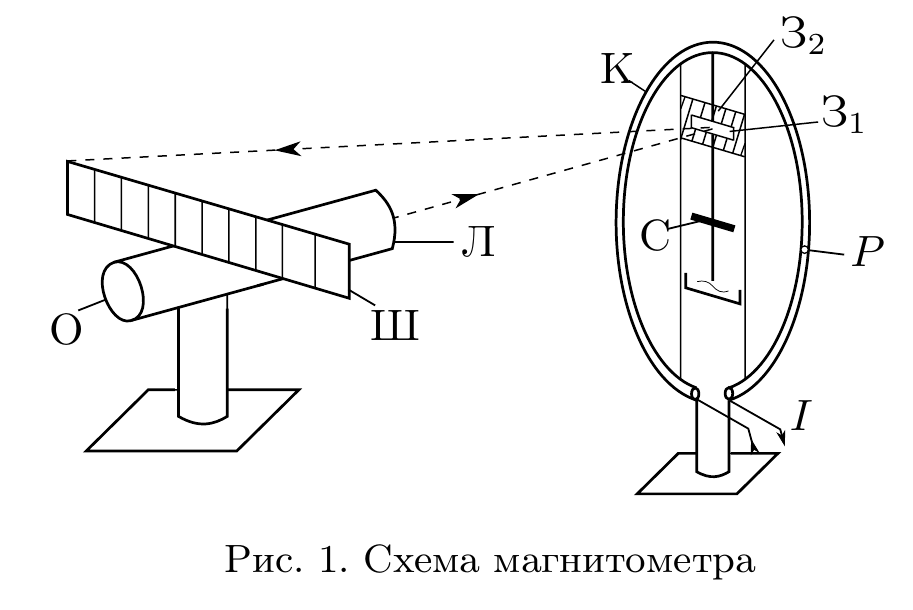
\includegraphics[width=0.8\linewidth]{../img/eq1.png}}
\end{figure}
Магнитометр состоит из нескольких последовательно соединённых круговых витков К, расположенных вертикально. В центре кольца К радиусом $R$ на тонкой неупругой вертикальной нити подвешена короткая магнитная стрелка С.  Жёстко связанная со стрелкой крыльчатка погружена в масло и служит для демпфирования колебаний.

\begin{figure}[ht!]
    \center{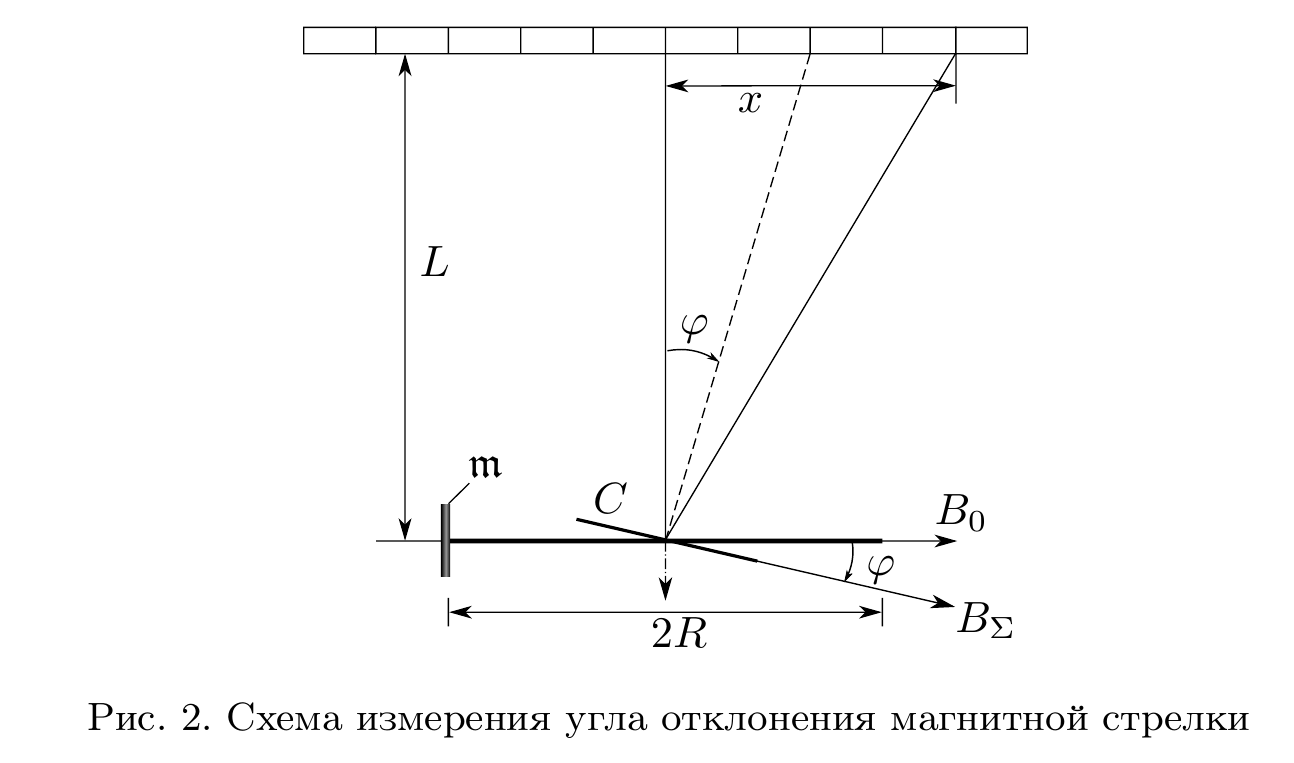
\includegraphics[width=0.8\linewidth]{../img/eq2}}
\end{figure}

В отсутствие других магнитных полей стрелка располагается по направлению горизонтальной составляющей земного магнитного поля $\vec{B_{0}}$. 

Прибор настраивают с помощью световых зайчиков, отражённых от двух зеркал: $\text{З}_{1}$, прикреплённого к стрелке (подвижный зайчик), и $\text{З}_{2}$, расположенного в плоскости кольца К и жёстко связанного с ним (неподвижный зайчик). Оба зеркала освещаются одним и тем же осветителем О. Вращением кольца вокруг вертикальной оси можно совместитьоба зайчика. При этом плоскость витков совпадает с плоскостью магнитного меридиана. При появлении дополнительного горизонтального магнитного поля $\vec{B}_{\bot}$ стрелка C установится по равнодействующей обоих полей $\vec{B_{ \Sigma}}$. В нашей установке дополнительное поле может быть создано либо малым ферромагнитным стержнем, расположенным на кольце на его горизонтальном диаметре, либо током, проходящим по кольцу.  В обоих случаях дополнительное поле можно считать однородным, так как размеры стрелки много меньше радиуса кольца.

Поле намагниченного стержня вдали от него может быть приближённо вычислено как поле точечного диполя:

\[
    \vec{B(\vec{r})} = \frac{ \mu_{0}}{4 \pi}\left(3\frac{\left(\vec{m}\cdot\vec{r}\right)\vec{r}}{r^{5}} - \frac{\vec{m}}{r^{3}}\right)
\]

На оси, перпендикулярной стержню
\[
    B_{1} = \frac{ \mu_{0}}{4 \pi}\frac{m}{R^{3}}
\]
$R$~--- радиус кольца.

Магнитное поле в центре кольца с током $I$
\[
    B_{2} = \frac{ \mu_{0} I}{2R} N
\]

\[
    B_{\bot} = B_{0}\tg \varphi
\]

Для определения горизонтальной составляющей земного магнитного поля $B_{0}$ тонкий короткий намагниченный стержень устанавливается в отверстие Р  на горизонтальном диаметре кольца. Измерив тангенс угла отклонения стрелки
\[
    \tg \varphi_{1} = \frac{x_{1}}{2L}
\]
можно рассчитать $B_{0}$.

Для исключения магнитного момента предлагается измерить период крутильных колебаний стержня в поле Земли. Подвешенный горизонтально за середину на тонкой длинной нити стержень в положении равновесия установится по полю Земли (упругость нити пренебрежимо мала). Если ось стержня отклонить в горизонтальной плоскости от направления $B_{0}$ на малый угол $ \alpha$, то под действием возвращающего механического момента
\[
    M_{\text{мех}} = mB_{0}\sin \alpha \approx mB_{0} \alpha
\]

Стержень с моментом инерции $J$ будет совершать крутильные колебания с периодом
\[
    T=2 \pi \sqrt{\frac{J}{mB_{0}}}
\]
Момент инерции цилиндрического стержня относительно оси вращения
\[
    J=m\left(\frac{l^{2}}{12} + \frac{r^{2}}{4}\right) = \frac{ml^{2}}{12}\left[1+3\left(\frac{r}{l}\right)^{2}\right]
\]
$m$~--- масса стержня, $l$~--- длина, $r$~--- радиус.

Тогда
\[
    B_{0} = \frac{2 \pi}{TR}\sqrt{\frac{ \mu_{0}JL}{2 \pi Rx_{1}}}
\]
Поскольку магнитометр установлен в железобетонном здании, магнитное поле в нём может не только сильно отличаться от поля Земли, но и заметно меняться от места к месту, поэтому период колебаний следует измерять непосредственно вблизи магнитометра. Кроме того, для обеспечения максимальной однородности магнитного поля в области измерений следует устранить (удалить на максимальное расстояние) возможные источники сильного магнитного поля: источники питания, токонесущие провода, сотовые телефоны, металлические предметы и т. п.

Ток в цепи кольца можно измерить двумя независимыми способами: по магнитному действию тока на стрелку магнитометра и по заряду, протекающему через цепь в единицу времени. Первый способ измерения соответствует тому, как эталон тока определён в системе СИ, а второй в гауссовой системе (СГС). По отношению результатов этих измерений можно определить электродинамическую постоянную $c$.

Пропуская некоторый ток через витки магнитометра, измерим тангенс угла отклонения стрелки $\tg \varphi_{2} = x_{2} / 2L$ и
\[
    I = \frac{2B_{0}R}{ \mu_{0}N}\tg \varphi_{2}
\]
Величина $A=2B_{0}R/ \mu_{0}N$  является постоянной прибора в данном месте земной поверхности (точнее, в данном месте комнаты — с учётом многочисленных сторонних источников магнитного поля).

Тот же ток можно измерить абсолютным образом по прошедшему в единицу времени заряду, что соответствует определению эталона тока в гауссовой системе (СГС). Если разрядить конденсатор известной ёмкости $C$, заряженный до напряжения $U$, через витки, то через них протечёт заряд $q=CU$. Если $ \nu$ раз в секунду последовательно заряжать конденсатор от источника и разряжать через витки, то через них за секунду протечёт заряд $CU\nu$, Средний ток. Средний ток, прошедший через витки, равен при этом
\[
    I=CU\nu
\]

Таким образом, абсолютное измерение тока сводится к нахождению величин $C$ и $U$, которые тоже могут быть определены абсолютным образом. Так, ёмкость плоского конденсатора можно вычислить из его размеров, то есть опираясь только на единицу длины. Разность потенциалов также может быть определена абсолютным образом, например, через силу, действующую на пластину заряженного конденсатора, как это делается в абсолютном вольтметре. Мы, однако, не будем полностью проводить эту программу, а ограничимся только указанием на возможность её выполнения.

Итак, для вычисления абсолютного значения тока необходимо измерить напряжение $U$ на конденсаторе известной ёмкости $C$. Напряжение необходимо выразить в единицах СГС ( $1\;\text{В}\approx \frac{1}{300}\;\text{ед. СГС}$). Ёмкость конденсатора  должна быть выражена в сантиметрах ($1\;\text{Ф}\approx 9\cdot 10^{11}\;\text{см}$).

По отношению численных значений одного и того же тока, выраженных в единицах СИ и СГС (гауссовой) , можно определить значение электродинамической постоянной:
\[
    c\left[\frac{\text{м}}{\text{с}}\right] = \frac{1}{10}\frac{I_{\left[\text{СГС}\right]}}{I_{\left[\text{СИ}\right]}}
\]

